\chapter{\label{ch:5-results}Results}


This section shows and discusses the results of our experiments based on the models and the datasets introduced in [methods section]. It also describes the rationale behind deciding which experiments should be run.

\section{HEXEvent dataset} \label{sec:hexevent}
To obtain a baseline, we evaluate the proposed models on the dataset from [dsc paper] as introduced in [section method hexevent dataset].

%1 AUC image with 4 models (nr 4 is DSC original) is enough; don't want to spend too much time on these results if I show that they are meaningless either way
%the table below will have concrete results either way

%---> doesn't really show how just bilstm is worse :(


\begin{figure}
	\centering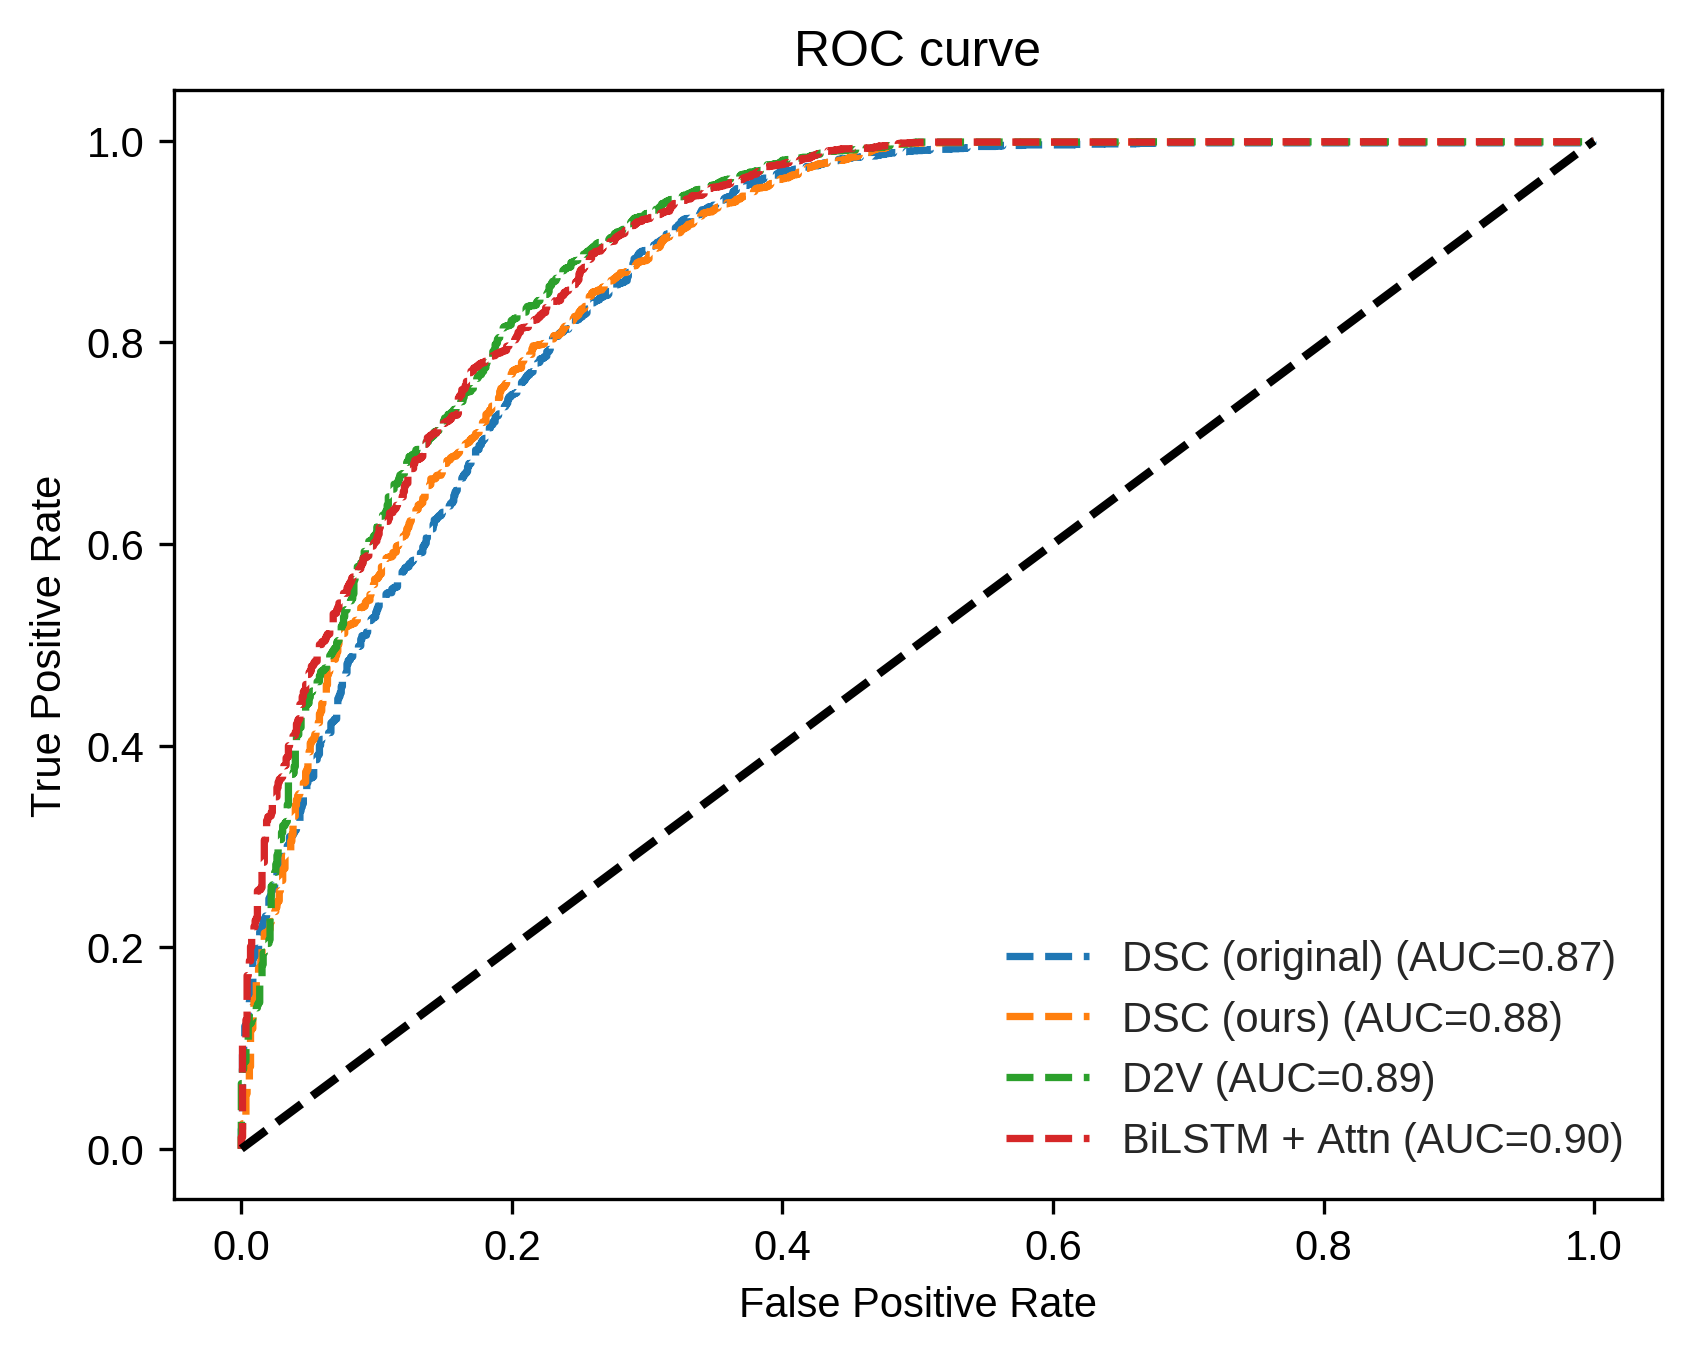
\includegraphics[width=0.7\textwidth]{../visualizations/hexevent_cross_model_roc_auc_comparison.png} 
	\caption[bla.]{Comparison of the ROC curves of the three main models (as well as the original implementation) on the HEXEvent dataset. }
	\label{fig:hexevent_auc}
\end{figure}

main takeaway: all models perform extremely well \& very similarly

%<discussion of results>
We are generally able to reproduce the performance of the DSC model of [dsc]. The 2\% performance difference between [dsc] and our re-implementation is likely just a result of random statistical noise influenced by random seeds and differences between TensorFlow / Keras (their model) and PyTorch (our model). Of our newly introduced models, the simple BiLSTM model performs worst.


%To showcase the advantage of using the attention mechanism, we also included the BiLSTM-based model where only the last output is used for classification. This model performs significantly worse than the other ones.

Observation: Performance heavily drops when no lengths feature is used


Reimplementation was done piece-wise, that is, first the sequence features were added as input, then the networks were trained to make sure that this was done correctly and then the length features were added. This lead to an interesting observation: model performance is significantly worse when no length features are given to the models. Quantitative results for this observation are given in table \ref{table:results_hexevent}.


\begin{table}[h!]
	\centering
	\begin{tabular}{| l | c | c | c| c} 
		\hline
		Model name & Only sequences & Sequences + lengths & Performance difference\\
		\hline
		DSC & 0.618 & 0.873 & 0.255\\
		D2V & 0.614 & 0.896 & 0.282\\
		BiLSTM + Attn & \textbf{0.636} & \textbf{0.904} & 0.268\\
		\hline
	\end{tabular}
	\caption{Performance of the main models on the HEXEvent dataset with and without length features given as AUC.  
	}
	\label{table:results_hexevent}
\end{table}


Concretely, [talk about exact quantitative results]\\

%Very surprisingly, model performance is almost invariant to whether sequence features are given or not!

To further stress test the dataset, we also test three other models: MLP100, MLP20 and MLPLinear which respectively contain 100, 20 and 20 trainable parameters. They are MLPs with only one hidden layer which only take the length features as inputs. MLPLinear doesn't use a non-linear activation function after its hidden layer.


\begin{figure}
	\centering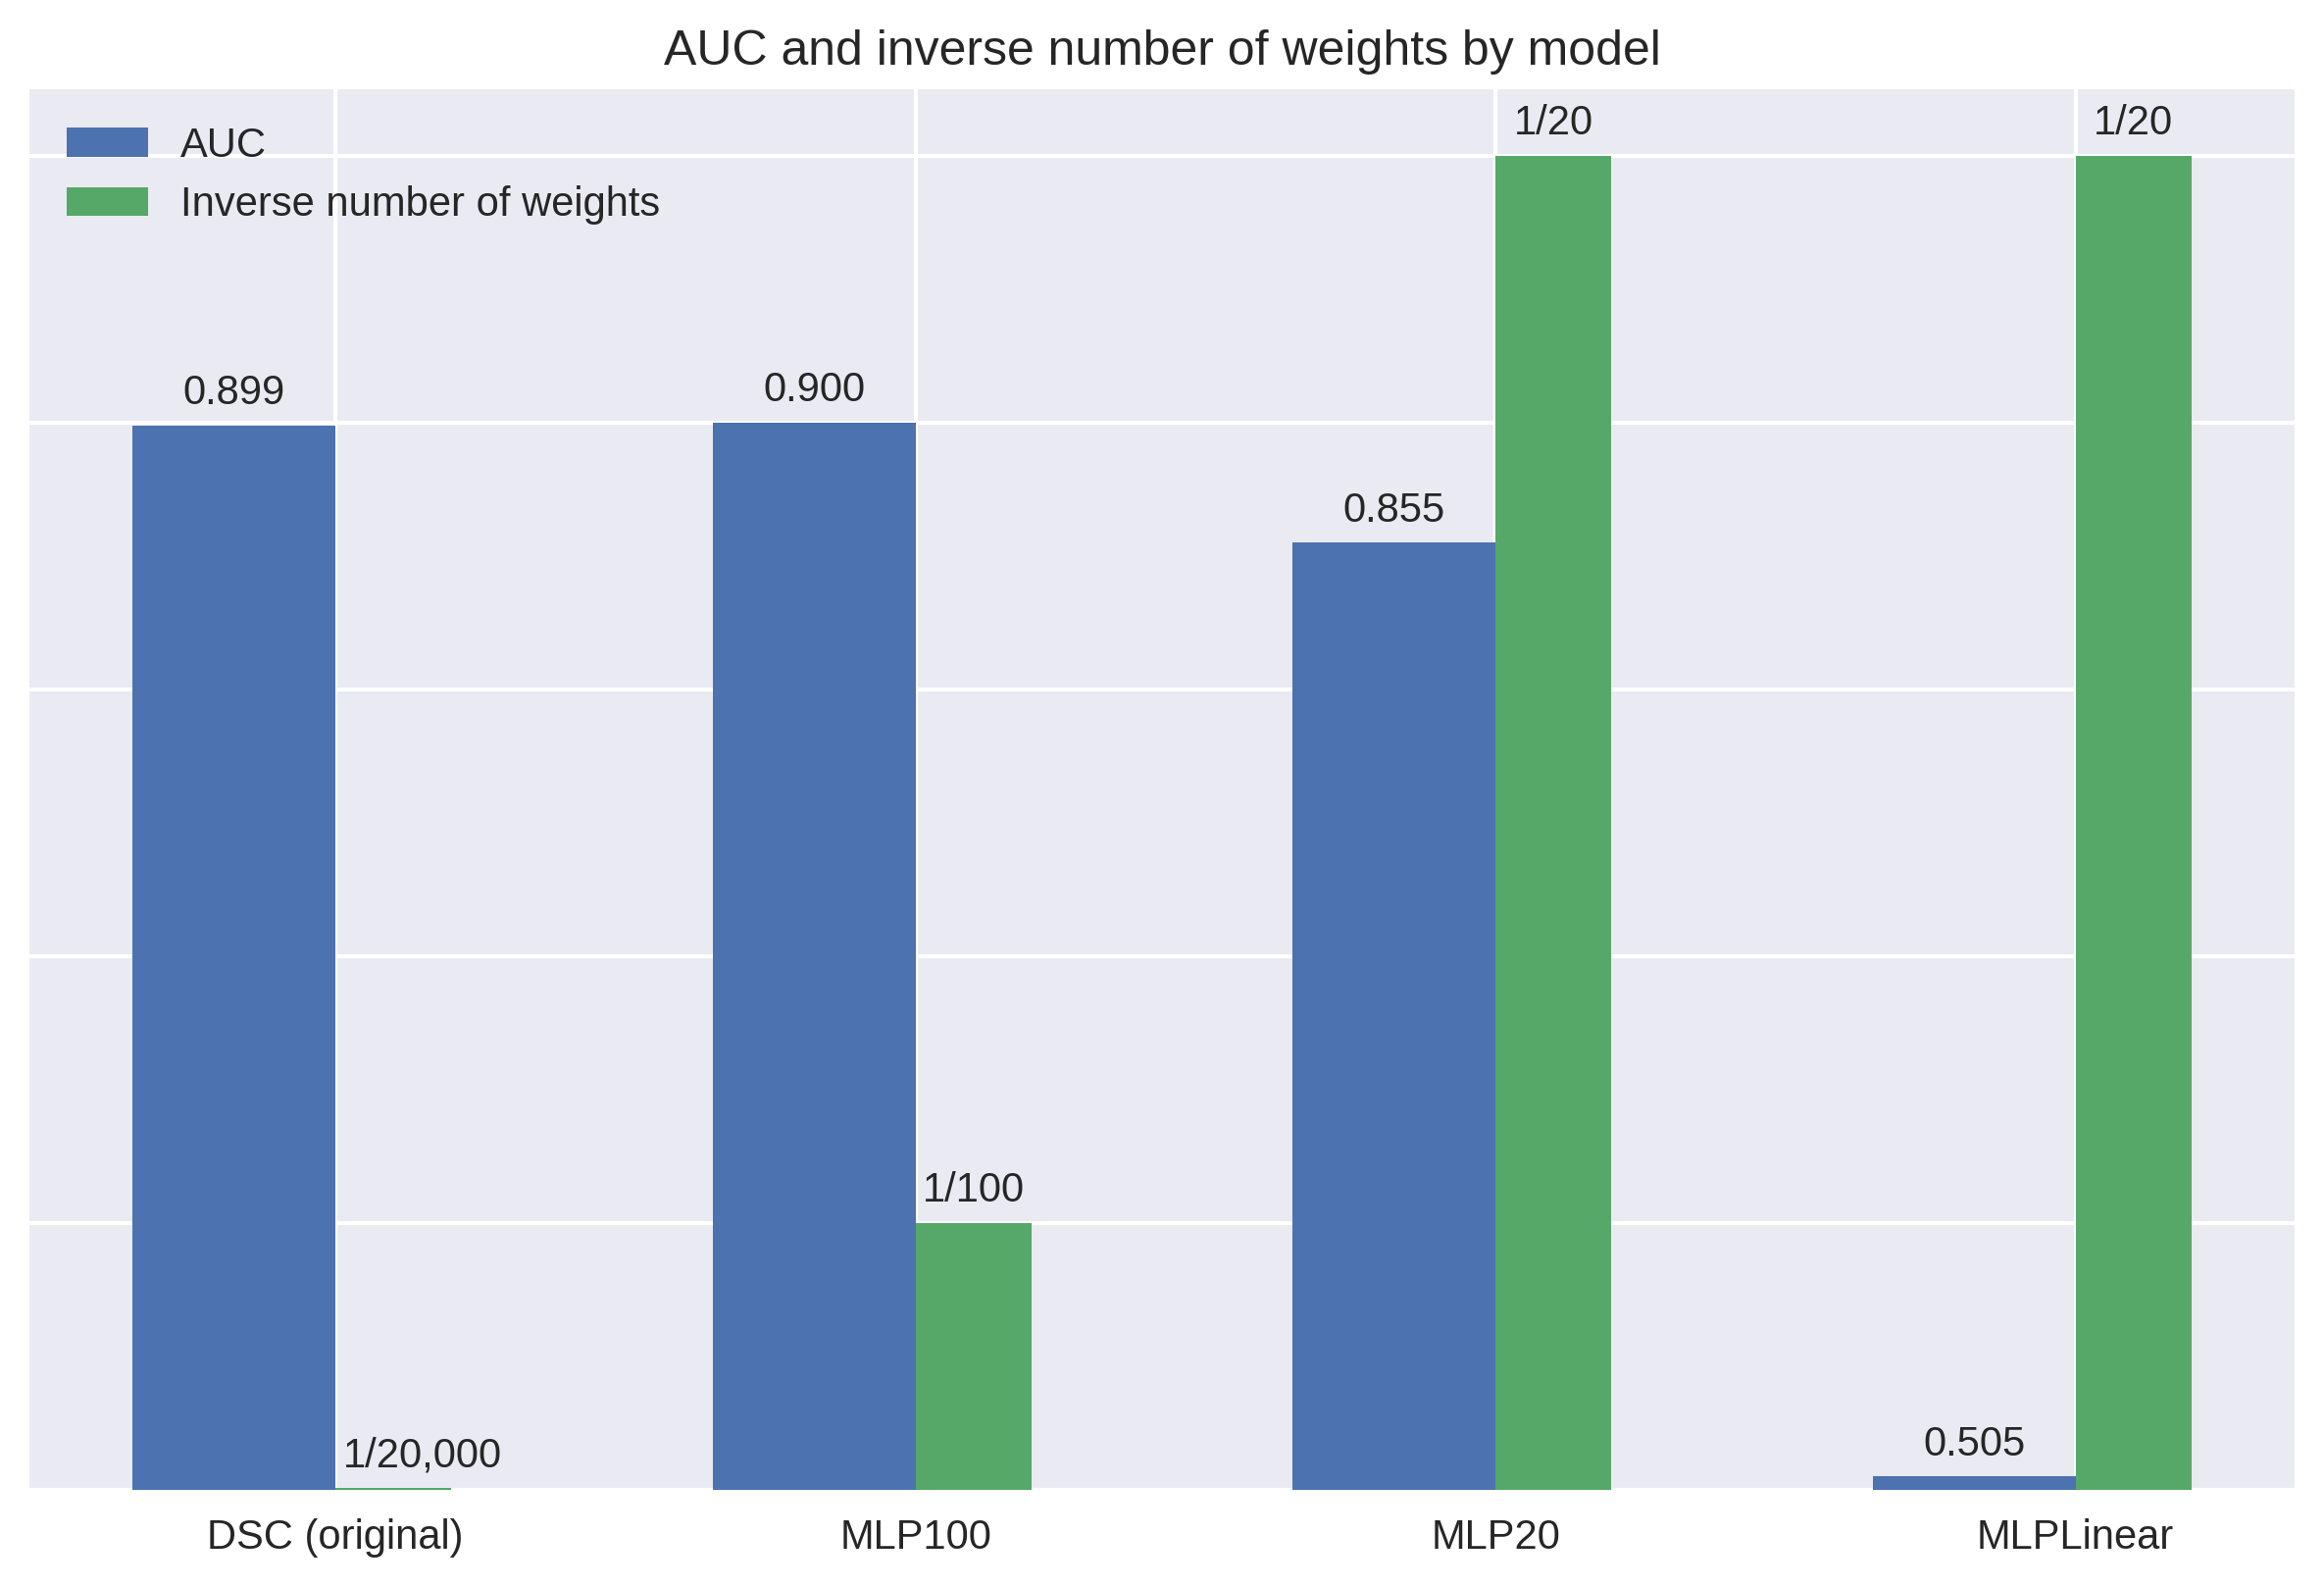
\includegraphics[width=0.7\textwidth]{../visualizations/dsc_funeral_barchart.png} 
	\caption[bla.]{Stress testing the HEXEvent dataset used in \cite{dsc}. The graph shows the performance as well as the inverse of the respective model sizes used.}
	\label{fig:dsc_funeral}
\end{figure}


The results in Figure \ref{fig:dsc_funeral} show that it is possible to replicate the results of \cite{dsc} with very simple models using two to three orders of magnitude fewer parameters. This indicates that a) either exon splicing is extremely well predictable based on the lengths of neighbouring introns and exons or 2) there are confounders in the dataset learned by the model.
Bugs in the replication (e.g. mixing of testing and validation data) are unlikely given that the same implementation was also able to reproduce [dsc papers]'s original results.
a) is extremely unlikely given that research into splicing has been ongoing for 50 years. a) can be disproven if this result fails to replicate on other datasets.
b) is substantially more likely, especially giving the discussions of biases in EST-based data. The biases inherent in EST-based data could be captured by the exon and intron structure and the model is learning to make its prediction based on this bias. b) can be shown if this result fails to replicate on other datasets. Model performance is improved by adding further parameters and breaks down when no non-linearities are used in the network. This indicates that there wasn't some mix-up during the data processing which would lead to even a linear model being able to predict alternative splicing, but that there is a non-trivial non-linear relationship which is being captured.
We showed that the EST-based HEXEvent dataset is likely too flawed to serve as a basis for our methods. Thus, we try to construct an alternative dataset.


\section{HipSci dataset}
\subsection{SUPPA with neurons}

\begin{figure}
	\centering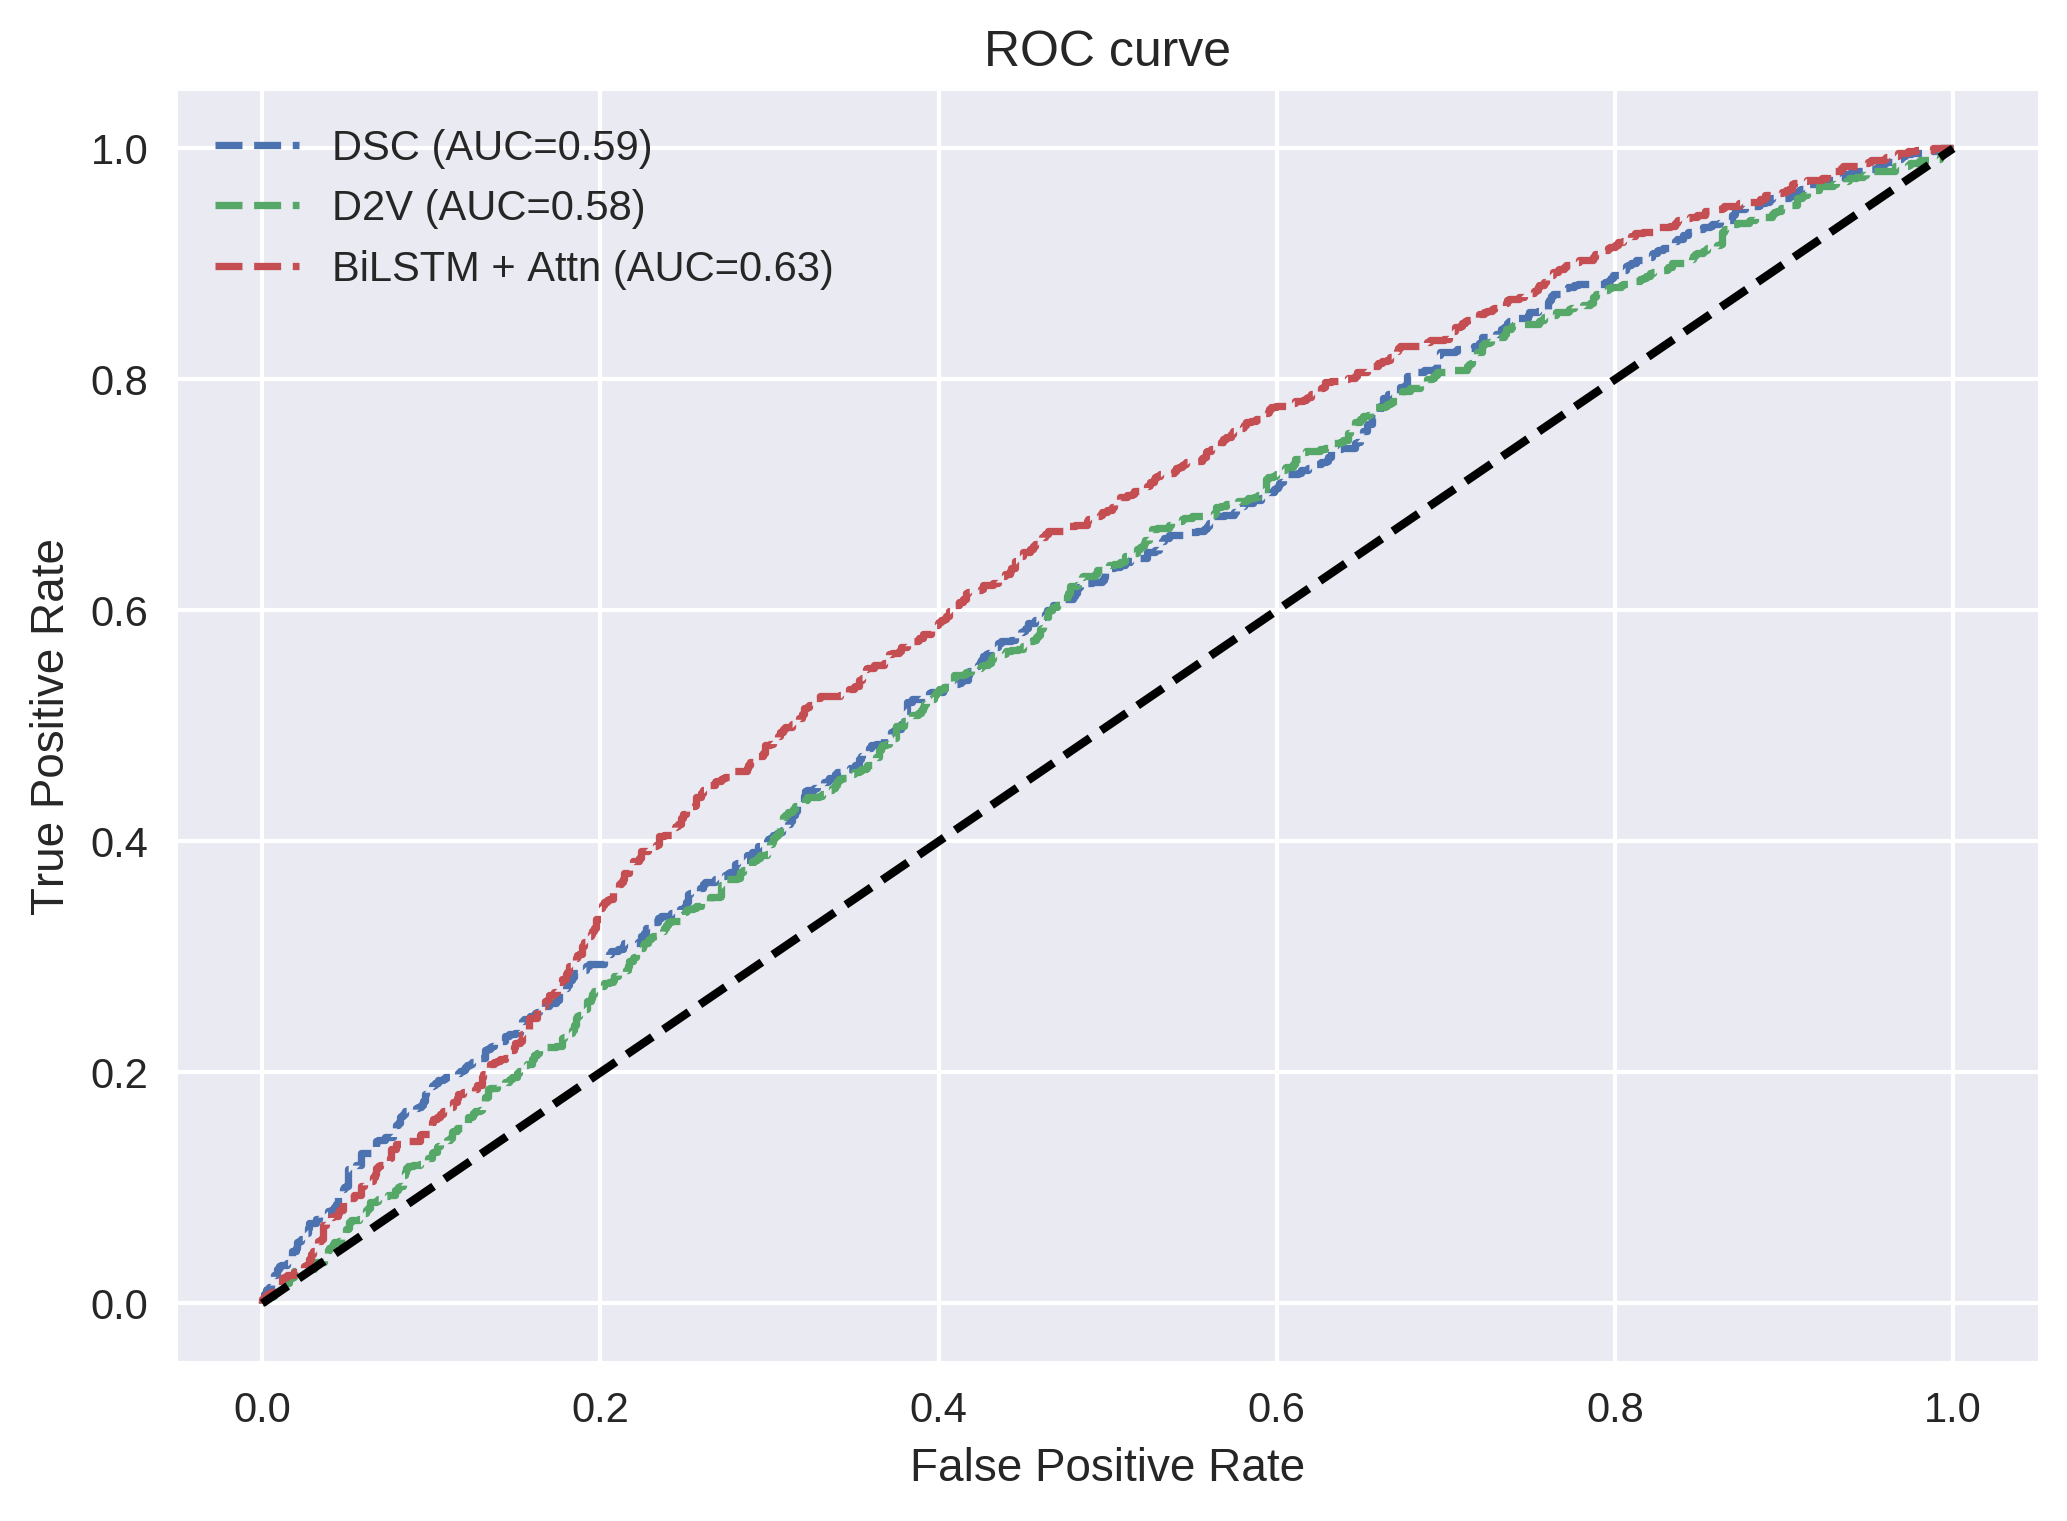
\includegraphics[width=0.7\textwidth]{../visualizations/suppa_cross_model_roc_auc_comparison.png} 
	\caption[bla.]{Comparison of the ROC curves of the three main models on the HipSci dataset derived by using SUPPA. }
	\label{fig:suppa_auc}
\end{figure}

Takeaways:
\begin{enumerate}
	\item All models perform similarly, BiLSTM + Attn tends to perform best
	\item All models perform very poorly perhaps a dataset issue (due to HIPSCI SUPPA being coarse-grained)
\end{enumerate}